\documentclass[12pt]{article}

\usepackage{graphicx}
\usepackage{grffile}
\usepackage{listings}
\usepackage{setspace}
\usepackage{color}
\usepackage{textcomp}
\usepackage[margin=1in]{geometry}
\usepackage[parfill]{parskip}
\usepackage{float}
\usepackage{vhistory}
\usepackage{caption}
\usepackage{subcaption}
\usepackage{tocloft}

\usepackage[]{hyperref}
\hypersetup{colorlinks=true,linkcolor=blue,urlcolor=blue}

% Definitions for Python code
\definecolor{Code}{rgb}{0,0,0}
\definecolor{Decorators}{rgb}{0.5,0.5,0.5}
\definecolor{Numbers}{rgb}{0.5,0,0}
\definecolor{MatchingBrackets}{rgb}{0.25,0.5,0.5}
\definecolor{Keywords}{rgb}{0,0,1}
\definecolor{self}{rgb}{0,0,0}
\definecolor{Strings}{rgb}{0,0.63,0}
\definecolor{Comments}{rgb}{0,0.63,1}
\definecolor{Backquotes}{rgb}{0,0,0}
\definecolor{Classname}{rgb}{0,0,0}
\definecolor{FunctionName}{rgb}{0,0,0}
\definecolor{Operators}{rgb}{0,0,0}
\definecolor{Background}{rgb}{0.98,0.98,0.98}

\renewcommand{\UrlFont}{\ttfamily\small}

\lstnewenvironment{PlainText}
    {\lstset{language=TeX,
        basicstyle=\ttfamily\scriptsize,
        upquote=true,
        linewidth=7in,
        frame=none, % frame=single
        }
    }
{}

\lstnewenvironment{Python}[1][]{
    \lstset{
        %numbers=left,
        %numberstyle=\footnotesize,
        %numbersep=1em,
        %xleftmargin=1em,
        %framextopmargin=2em,
        %framexbottommargin=2em,
        showspaces=false,
        showtabs=false,
        showstringspaces=false,
        frame=none, %frame=single,
        tabsize=4,
        % Basic
        basicstyle=\ttfamily\scriptsize,
        backgroundcolor=\color{Background},
        language=Python,
        upquote=true,
        % Comments
        commentstyle=\color{Comments}\slshape,
        % Strings
        stringstyle=\color{Strings},
        morecomment=[s][\color{Strings}]{"""}{"""},
        morecomment=[s][\color{Strings}]{'''}{'''},
        % keywords
        morekeywords={import,from,class,def,for,while,if,is,in,elif,else,not,and,or,print,break,continue,return,True,False,None,access,as,,del,except,exec,finally,global,import,lambda,pass,print,raise,try,assert},
        keywordstyle={\color{Keywords}\bfseries},
        % additional keywords
        morekeywords={[2]@invariant},
        keywordstyle={[2]\color{Decorators}\slshape},
        emph={self},
        emphstyle={\color{self}\slshape},
        linewidth=7.1in, % extra-width for source code
        %
    }
}{}

\begin{document}

\title{dstauffman User's Guide}
\author{David C. Stauffer}
\date{August 3, 2015}
\maketitle

\begin{abstract}\label{Abstract}
The first half of this document is meant to be a simple guide to get someone up and running the dstauffman library, describing it's main use cases and functionality.  The second half of the document is targeted towards future developers of the code.  It covers layout, documentation guidelines, unit test cases and code coverage philosophies and how to go about potentially contributing to the source.
\end{abstract}

\begin{versionhistory}
    \vhEntry{--}{2015-08-03}{DCS}{Initial Release.}
\end{versionhistory}
\addcontentsline{toc}{section}{Revision History}

\pagebreak
\tableofcontents
\addcontentsline{toc}{section}{Contents}

\pagebreak
\listoffigures
\addcontentsline{toc}{section}{List of Figures}
\listoftables
\addcontentsline{toc}{section}{List of Tables}

\pagebreak
\section{User's Guide to the Code}\label{h1:Users_guide}
\subsection{Retrieving the Library}\label{h2:Retrieving_the_library}
The master repository of the source code is currently hosted on GitHub at:
\newline\url{https://github.com/DStauffman/dstauffman}

The repository is public, so anyone can access it through github.com even without an account.  To do pull requests to potential modify the code and have your changes incorporated in a future version, then you'll need to have a GitHub account.  You can join for free by going to:
\newline\url{https://github.com/join}

\subsection{Installing Python}\label{h2:Installing Python}
The dstauffman library is written in Python 3.4.  It relies heavily on the numpy and matplotlib libraries along with Sphinx for auto-documentation generation using the numpydoc standard.  The code is developed on Windows 7 using WinPython (currently v3.4.3.3).  It is intended to be platform independent with Unix/Mac (but is rarely tested on those platforms), and also backwards compatible with Python 2.7 (tested with WinPython v2.7.9.3).

In order to run the code, you'll need an appropriate version of Python installed along with numpy and matplotlib.  If you are on Unix, you probably have this already.  If you are on Windows, then I highly recommend the WinPython distribution available at:
\newline\url{http://winpython.sourceforge.net/}

The WinPython distribution automatically includes all the libraries you'll use, plus the Spyder IDE and/or IPython, which can give you a very MATLAB-like interface.  It can be installed to any folder location without admin rights, and you can simultaneously install multiple versions and easily run them without conflicts.  More details on some of my favorite Spyder and Python tweaks are include in Section~\ref{h3:Spyder_install}.

\subsection{Preparing Python}\label{h2:Preparing_python}
The code is designed to be imported as a library.  In order for that to happen, the ``dstauffman'' folder must be on your python path.  The easiest way (but not the recommended way) to do this is to copy the folder into the existing Python library location.  If you install WinPython to the root C: drive within a ``Programs'' folder, then this might be somewhere like:
\newline\url{C:/Programs/WinPython-64bit-3.4.3.3/python-3.4.3.amd64/Lib}

The recommended method is to modify your user ``PYTHONPATH'' variable.  On Windows 7, you can do this by hitting start, and then starting to type ``environment'' and choosing the ``Edit environment variables for your account'' within the control panel.

\begin{figure}[H]
    \centering
    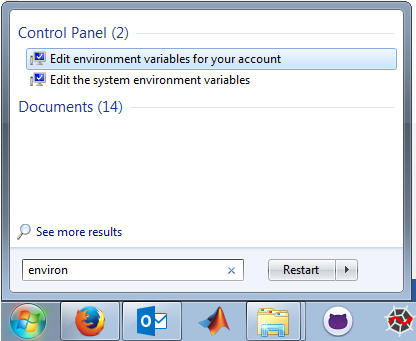
\includegraphics[width=.6\textwidth]{Environment_Variables1.png}
    \caption{Editing your PYTHONPATH variable, step 1.}
    \label{fig:environment1}
\end{figure}

Then if the user variable for ``PYTHONPATH'' (one word, all caps) doesn't exist, create a new one. If it does, append to it.  On Windows use a semi-colon (;) to separate folders, and on Unix, use a colon (:) and don't put any spaces between folders.  Add the folder location that contains the ``dstauffman'' folder.  In my case, that's the GitHub folder where I keep my local copy of the repository.

\begin{figure}[H]
    \centering
    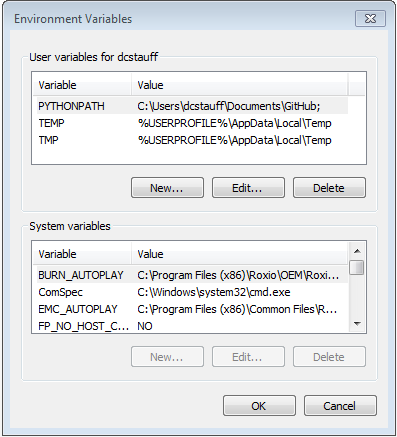
\includegraphics[width=.6\textwidth]{Environment_Variables2.png}
    \caption{Editing your PYTHONPATH variable, step 2.}
    \label{fig:environment2}
\end{figure}


\subsection{Running the Code}\label{h2:Running_the_code}
At least one example script should be available in the /dstauffman/scripts folder.  This script can be run via a command prompt:
\begin{PlainText}
python script_name.py
\end{PlainText}

If you are on Windows and installed WinPython as described earlier, then python may not be on your system path, and you'll likely need to fully qualify the names:
\begin{PlainText}
"C:\Programs\WinPython-64bit-3.4.3.3\python-3.4.3.amd64\python.exe" 
  "C:\Users\dcstauff\Documents\GitHub\dstauffman\scripts\example_script.py"
\end{PlainText}

\begin{figure}[H]
    \centering
    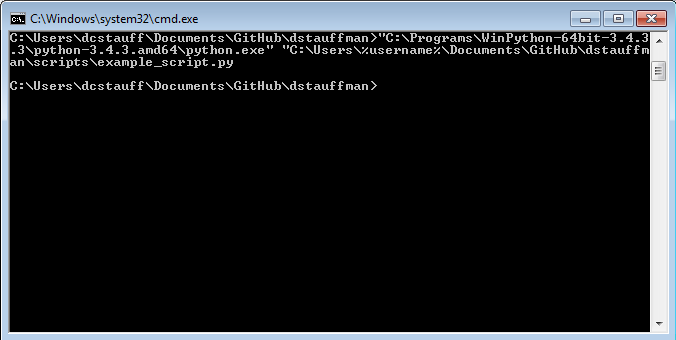
\includegraphics[width=\textwidth]{Running_Code_via_cmd.png}
    \caption{Running a script via command prompt.}
    \label{fig:running_via_cmd}
\end{figure}

If you want to be able to interact with the results or the plots, then the better way to run the script is by opening it within Spyder and running it in that application.  Spyder can run a normal console or IPython console.  The IPython one has a lot of advantages, but I've found that it also causes some weird bugs and instabilities, so if you are just getting up and running, then I recommend a normal console window.

\begin{figure}[H]
    \centering
    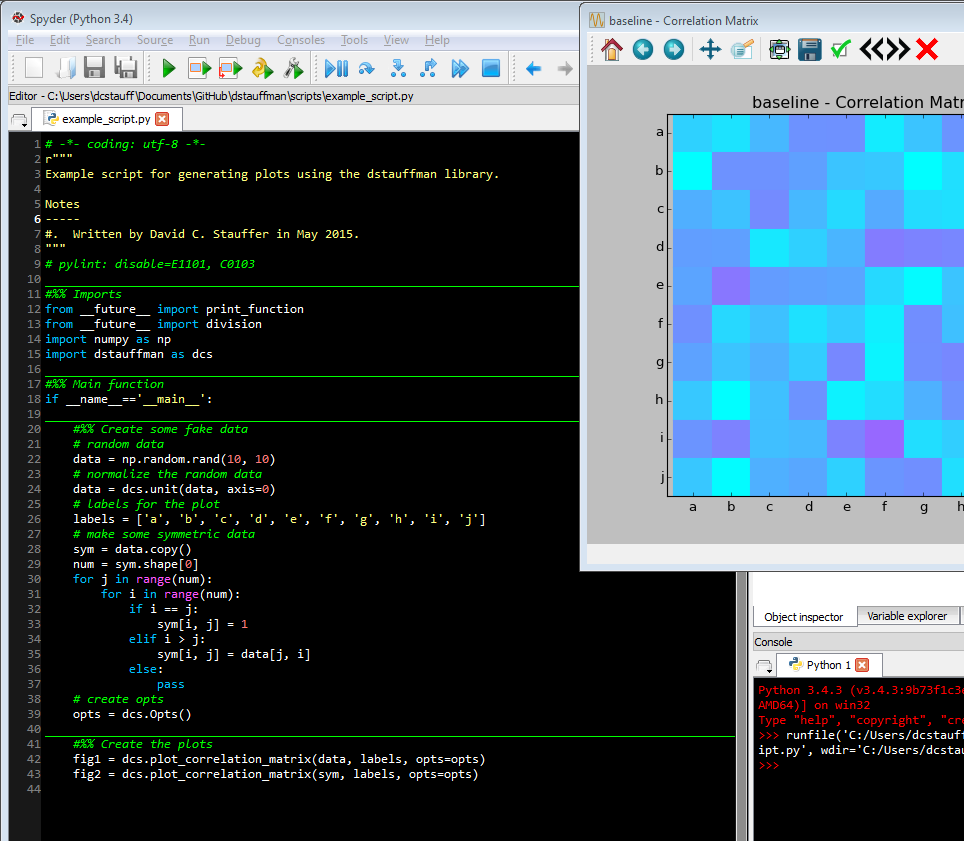
\includegraphics[width=\textwidth]{Spyder_IDE_screenshot.png}
    \caption{Example of opening and executing the example\_script.py within Spyder.}
    \label{fig:spyder_example}
\end{figure}

\subsection{Explanation of Script}\label{h2:Explanation_of_script}
The first key part of the script are the import statements, namely the one where the dstauffman library is imported:
\begin{Python}
    import dstauffman as dcs
\end{Python}

\textcolor{red}{TODO.}

\subsection{Further Code Documentation}\label{h2:Further_code_documentation}
The specific functions and classes within the code are intended to be self-documented within the source.  This is the best way to ensure that the documentation stays current with the code.  For easier distribution purposes, this in-source documentation (the so-called Python docstrings) can be automatically compiled into an html guide.  The current version of this documentation is available at ./dstauffman/doc/build/dstauffman.html.  See Section~\ref{h2:autodoc} for more details.

\pagebreak
\section{Developer's Guide to the Code}\label{h1:Developers_guide}
This section goes into more detail about the layout, documentation, code coverage, test cases and design philosophies.  It is intended to let other future potential developers of the library know what choices I made and why, allowing their use to continue and expand.

\subsection{Basic Code Layout}\label{Basic_code_layout}
The code is intended to be imported as a single module, but for organization and readability purposes, it is split into a number of different files.  The high-level description of these is as follows:
\begin{itemize}
    \setlength{\itemsep}{0pt}
    \setlength{\parskip}{0pt}
    \setlength{\parsep}{0pt}
    \item \_\_init\_\_.py - Does relative imports so that the entire module can be imported with just one ``import dstauffman'' command.
    \item classes.py - Contains the high level classes used throughout the rest of the library.
    \item constants.py - Defines constants used throughout the rest of the library.
    \item enums.py - Defines enumerators used by the rest of the library.
    \item photos.py - Contains routines for managing pictures and images.
    \item plotting.py - Defines plotting functions to display the results from the rest of the model.
    \item quat.py - Contains quaternion (and some vector) related math routines.
    \item utils.py - Contains generic utilities that can be independently defined and used throughout the rest of the library.
\end{itemize}

In addition, there are a couple other files at the root level.  These are used as follows:
\begin{itemize}
    \setlength{\itemsep}{0pt}
    \setlength{\parskip}{0pt}
    \setlength{\parsep}{0pt}
    \item .gitattributes - Used to config things about the Git repository.  Currently it doesn't do much.
    \item .gitignore - Used to control what items are ignored by the change tracking.  There are a lot of lines in here to ignore temp windows and/or Python files, along with \LaTeX build files and also temporary and results output folders.
    \item LICENSE.txt - Defines the license to be used by anyone who wants to take the source code and use or modify it for their own purposes.  I chose the LGPL v3 license because the code is being developed as a software library package and this is otherwise an extension of the popular GPL license.  It allows commercial usage, but requires anyone who modifies the code to share their source under the same license.  If they use the code without modification, then they don't have this restriction.  (See \href{http://choosealicense.com/}{choosealicense.com} for details)
    \item README.txt - Read me file for use on GitHub, it generally contains the same high level information that is at the top of the \_\_init\_\_.py file.
\end{itemize}

In addition to all the files, there are subfolders within the repository.  These are used as follows:
\begin{itemize}
    \setlength{\itemsep}{0pt}
    \setlength{\parskip}{0pt}
    \setlength{\parsep}{0pt}
    \item .git - Hidden folder used by Git for all the change tracking.
    \item \_\_pycache\_\_ - Folder used by Python v3+ for object/byte code.  (In Python v2.7, this code goes into the same folder as the source. I prefer the breakout that Python v3 does much better)
    \item archery - Folder that contains archery related submodules, meant to be imported separately
    \item data - Folder that contains data files, mostly just a place holder for now.
    \item doc - Folder for code documentation.  The main documents are in there at the root doc level, along with further subfolders for other documents.  The build and source subfolders are used by Sphinx for autodocumentation, and the tex folder for organizing the code to generate the \LaTeX\ pdf documents.
    \item games - Folder that contains gaming related submodules, meant to be imported separately.  Currently it has one game, brick.
    \item images - Folder that contains image files (*.jpg, *.png, etc.) for use in the rest of the library.
    \item output - Folder used to store output files.  It is ignored by the Git repository.
    \item results - Another Folder used to store output files.  It is ignored by the Git repository.
    \item scripts - Folder used to contain scripts.  Some are tracked as example templates, but anything that starts with ``script\_'' or ``case\_'' is currently ignored by Git.
    \item support - Folder of Python code that is used in a supporting sense.  So code that generates other code, or looks for things to be merged within other code libraries back into this library.
    \item temp - Convenient folder to dump temporary files into.  Everything in here is ignored by Git.
    \item tests - Folder containing the unit test cases and the .coveragerc configuration file.  When the code coverage test is run, the results also go here into a ``coverage\_html\_report'' subfolder.
\end{itemize}

\subsection{Autodocumentation with Docstrings and Sphinx}\label{h2:autodoc}
The code is as much as possible self-documented.  This is achieved through the use of docstrings within the Python source code.  The docstring is the first continuous block of comments following a ``def'' or ``class'' definition.  See more details about Python docstrings in \href{https://www.python.org/dev/peps/pep-0257/}{PEP-257}.

Including the documentation as part of the source code is the best way to try and enforce that they stay consistent with one another.  It still requires an author to check the comments when they are making changes to the code, but it's much easier for them to do that right there on the same screen than trying to remember to go to some other file and see if it needs to be updated.

\subsubsection{Sphinx and numpydoc}
One problem that occurs with in-source documentation, is that some users of the model may not care about the source code details, but still want to read the documentation.  This is where Sphinx comes in.  Sphinx allows you to automatically generate HTML documentation directly from the docstring comments.  This documentation is hyperlinked to all the different module functions and includes input and output parameter descriptions (as listed in the source code).  The Sphinx autogenerated documentation is available in the repository at: ./dstauffman/doc/build/dstauffman.html

The built-in Python standard for these are somewhat limited, so I use the much more robust numpydoc standard that was developed and used within the numpy library.  numpy is \emph{the} numerical analysis library that does almost all of the computation within the model, so I like following their standard.  It is documented here: \url{https://github.com/numpy/numpy/blob/master/doc/HOWTO_DOCUMENT.rst.txt} with a good example file here: \url{https://github.com/numpy/numpy/blob/master/doc/example.py}

In general, the more information you put into the docstrings, the better.  At a minimum, it should have a one line summary of the function.  A list of all the inputs in a ``Parameters'' section.  Any specific outputs in a ``Results'' section.  A ``Notes'' section with the change history plus any other useful information, such as any variables modified in place, plus an ``Examples'' section with at least one complete example for how to execute the function.  This example is written in the ``doctest'' format that allows it to be automatically executed as an additional unit test.  This extra test is redundant with the more complete unittests, but ensures that the example given will actually execute.  The doctest library is described more here: \url{https://docs.python.org/3.4/library/doctest.html}

Running the ./dstauffman/tests/run\_all\_docstrings.py script will execute all the doctests within the code.  An example function header is shown below:

\begin{Python}
def rms(data, axis=None, keepdims=False):
    r"""
    Calculates the root mean square of a number series

    Parameters
    ----------
    data : array_like
        input data
    axis : int, optional
        Axis along which RMS is computed. The default is to compute the RMS of the flattened array.
    keepdims : bool, optional
        If true, the axes which are reduced are left in the result as dimensions with size one.
        With this option, the result will broadcast correctly against the original `data`.

    Returns
    -------
    out : ndarray
        RMS results

    See Also
    --------
    numpy.mean, numpy.conj, numpy.sqrt

    Notes
    -----
    #.  Written by David C. Stauffer in Mar 2015.

    Examples
    --------

    >>> from dstauffman import rms
    >>> rms([0, 1, 0., -1])
    0.70710678118654757

    """
\end{Python}

One exception to this more complex docstring header would be a very simple class definition, such as a enumerator, or a method to a larger class.  These often only have a single line docstring.  A simple example is shown below for the list\_of\_names method within the custom \_EnumMetaPlus class.

\begin{Python}
    def list_of_names(self):
        r"""
        Returns a list of all the names within the enumerator.
        """
        output = re.findall(r"\.(.*):", str(self))
        return output
\end{Python}

\subsubsection{Bulding Sphinx documentation}
To generate the documentation, use the ``sphinx-build'' command.  If Sphinx is not automatically a part of your Python installation, then you can install it through ``pip``. See \url{http://sphinx-doc.org/latest/install.html} for more information.
\begin{PlainText}
pip install sphinx
\end{PlainText}

Once Sphinx is installed, then it's a one line build command.  This command tells Sphinx to build the HTML documentation using the specified source folder into the specified build folder.
\begin{PlainText}
sphinx-build -b html source_folder build_folder
\end{PlainText}

The details controlling what gets documented are in the ./dstauffman/doc/source subfolder.  The ``conf.py'' file controls the Python side of things, and the 3 *.rst files (dstauffman.rst, index.rst, and modules.rst) build the tree layout to traverse.  If you add a new function or class definition to an existing submodule file, then nothing special needs to be done to include it in the next Sphinx build.  If you create a brand new submodule, then you'll need to modify the ``dstauffman.rst'' file.  Using the existing lines as a template and it should be pretty clear what to add.  If you want to update the version number within the documentation, then that gets changed within the ``conf.py'' file (or as an optional additional parameter to the build command).

\subsection{Unit Tests}\label{h2:Unit_tests}
One of the major efforts for this code has been developing comprehensive unit test cases for all the functions.  This takes extra time and work up front, but in my mind pays back tremendously in the long run.  It helps flush out bugs much earlier in the design cycle, prevents you from getting to more complicated bugs, and signficantly increases my confidence that the code does what it was designed to do.  It will likely never flush out all the bugs, but hopefully goes a long way towards that goal.

The unit tests are defined and executed using the Python ``unittest'' library.  You can get more information about it here: \url{https://docs.python.org/3/library/unittest.html}

In general, there is a Test\_xxxx class defined as a subclass of unittest.TestCase, with optional setUp and tearDown methods to create variables and do initializations, and then any test\_yyyy method is a specific unit test.  Each unittest should be targeted towards one specific variation of the code.  They should be simplified test cases such that the answer can be known or intuited beforehand.  For example, the rms function is basically implemented in a single line of Python code, but covers a lot of different use cases with different complications.

To test this function, all the different inputs are used one at a time, a scalar, a vector and a matrix with numbers such that the RMS can be calculated manually and known beforehand.  Additionally, each optional parameter is testing with their different values, so in this case with axis not specified, or specified as the first or last dimension, and then with the keepDims variable true or false.  The rms function is also defined for complex numbers, so those are tested.

With all of these combinations, it's sometimes hard to know what doesn't need to be tested.  For instance, a separate int case is not included, because they will convert to floats as necessary.  Additionally a bad axis case is not included, because the function is meant to mimic the np.mean function, so that function will catch the error for us in whatever it's normal behavior is.

\begin{Python}
#%% rms
class Test_rms(unittest.TestCase):
    r"""
    Tests the rms function with these cases:
        rms on just a scalar input
        normal rms on vector input
        rms on vector with axis specified
        rms on vector with bad axis specified
        rms on matrix without keeping dimensions, no axis
        rms on matrix without keeping dimensions, axis 0
        rms on matrix without keeping dimensions, axis 1
        rms on matrix with keeping dimensions
        rms on complex numbers
        rms on complex numbers that would return a real if done incorrectly
    """
    def setUp(self):
        self.inputs1   = np.array([0, 1, 0., -1])
        self.outputs1  = np.sqrt(2)/2
        self.inputs2   = [[0, 1, 0., -1], [1., 1, 1, 1]]
        self.outputs2a = np.sqrt(3)/2
        self.outputs2b = np.array([np.sqrt(2)/2, 1, np.sqrt(2)/2, 1])
        self.outputs2c = np.array([np.sqrt(2)/2, 1])
        self.outputs2d = np.matrix([[np.sqrt(2)/2], [1]])

    def test_scalar_input(self):
        out = dcs.rms(-1.5)
        self.assertEqual(out, 1.5)

    def test_rms_series(self):
        out = dcs.rms(self.inputs1)
        self.assertAlmostEqual(out, self.outputs1)

    def test_axis_drop1a(self):
        out = dcs.rms(self.inputs1, axis=0)
        self.assertAlmostEqual(out, self.outputs1)

    def test_axis_drop1b(self):
        with self.assertRaises(IndexError):
            dcs.rms(self.inputs1, axis=1)

    def test_axis_drop2a(self):
        out = dcs.rms(self.inputs2)
        self.assertAlmostEqual(out, self.outputs2a)

    def test_axis_drop2b(self):
        out = dcs.rms(self.inputs2, axis=0, keepdims=False)
        for (ix, val) in enumerate(out):
            self.assertAlmostEqual(val, self.outputs2b[ix])

    def test_axis_drop2c(self):
        out = dcs.rms(self.inputs2, axis=1, keepdims=False)
        for (ix, val) in enumerate(out):
            self.assertAlmostEqual(val, self.outputs2c[ix])

    def test_axis_keep(self):
        out = dcs.rms(self.inputs2, axis=1, keepdims=True)
        for i in range(0, len(out)):
            for j in range(0, len(out[i])):
                self.assertAlmostEqual(out[i, j], self.outputs2d[i, j])

    def test_complex_rms(self):
        out = dcs.rms(1.5j)
        self.assertEqual(out, np.complex(1.5, 0))

    def test_complex_conj(self):
        out = dcs.rms(np.array([1+1j, 1-1j]))
        self.assertAlmostEqual(out, np.sqrt(2))
\end{Python}

\subsection{Code Coverage}\label{h2:Code_coverage}
One of the most key aspects of good unit testing is that it covers all possible lines of the code.  If there is an if/else block, then you need a test that covers the if condition, and another test that covers the else condition.  Determining this manually can be very difficult, so Python has the ``coverage`` library that allows us to do it automatically.  Running the coverage report tool will generate a table like the one shown in Figure~\ref{fig:code_coverage}.  This is an HTML report, so each file can be clicked, and then it will shown a line by line breakdown, with color codes to show which lines were executed, which were ignored, and which ones were never executed.  This report can be generated via a couple commands.  One to run the analysis, one to generate the report, and then for convenience, one to open the report:
\begin{PlainText}
cd C:\Users\%username%\Documents\GitHub\dstauffman\tests
coverage run run_all_tests.py
coverage html
start C:\Users\%username%\Documents\GitHub\dstauffman\tests\coverage_html_report\index.html
\end{PlainText}

The report results themselves are not saved within the repository, so you will need to re-run the test to view them.  There is one configuration file at ./dstauffman/tests/.coveragerc that is part of the repository that controls which files are ignored.  For instance, you don't want the test report to show you the coverage results on the tests, but only on the functions they are testing.

\begin{figure}[H]
    \centering
    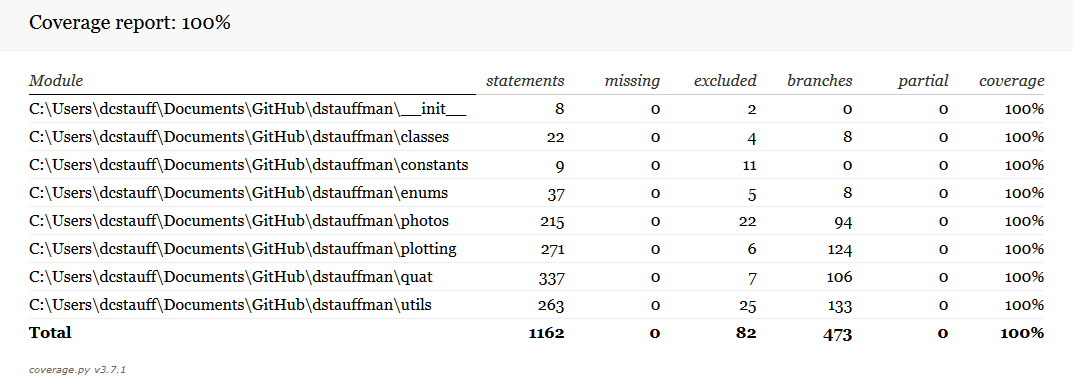
\includegraphics[width=\textwidth]{Coverage.png}
    \caption{Code coverage statistics.}
    \label{fig:code_coverage}
\end{figure}

\subsection{GitHub Repository Details}\label{h2:github_details}
As stated in the very beginning of this document, the source code is hosted in a GitHub repository at:
\url{https://github.com/DStauffman/dstauffman}

\subsubsection{Branches}
My goal is to always have the ``master'' branch within Git be a working, stable version of code.  However, developers need a playground to make changes that might not be complete, so there are development branches.  Currently I'm developing on the ``0.x\_dev'' branch.  Once I release a v1.0 code base, then I'll migrate to a ``1.x\_dev'' branch and so on.  I do the work on the development branch, and when it gets far enough to be a substantial improvement, then I go through a whole round of testing, update the Sphinx documentation, make a tag, and then merge the branch into ``master''.

\subsubsection{Tags}
Tags allow you to quickly pull up the specific version of code that was tagged.  These are useful checkpoints to make every 2-3 weeks.  I try to always do a good round of testing, such that the tags will fully execute without bugs.  Sometimes the tags are on the development branch, and sometimes on the master, depending on need.  To make a tag, use this command with the appropriate version number.

\begin{PlainText}
git tag -a v1.0.0 -m 'Tag comments'
\end{PlainText}

Release tags also allow users to go on github.com and download a zip file with just the contents of the specific tag.  So if you have results published with a v0.1.0 tag, then anyone can grab that specific version of code, and hopefully run it to reproduce the results.  I use a three digit version number, so the last digit is for minor changes released more based on time.  The middle digit for big points that should be captured, and the first digit for major milestones, such as published papers or entirely new disease models.

Additionally, you can create a branch using the ``git branch'' command or switch to a branch using the ``git checkout'' command.  Both of these steps can also easily be done through the GitHub for Windows application.

\subsubsection{Merging}
Merging a branch is slightly more difficult.  There are also multiple ways to merge a branch, depending if you want all the sub-commits preserved or if you want it done in one large piece.  I've been doing sub-commits, but will likely switch to large single commits on the master branch in the future, and then always keep the development branches around for the details.

Basically to do a merge you need to commit things on the development branch, switch to the master, merge stuff in, commit (or push) the merged changes on the master branch, and then if applicable, switch back to the development branch.  Via command prompt, it's something like this:
\begin{PlainText}
git checkout master
git merge branchname
git push
git checkout branchname
\end{PlainText}

\subsection{Miscellaneous Lessons Learned}\label{h2:misc_lessons}
I've learned some random but useful tips and tricks along the way.  This section is used to capture them.

\subsubsection{Enums}
For states with a small number of discrete possibilities I strongly recommend using enumerators instead of just a simple numeric value.  The enumerator adds a level of autodocumentation that is useful, plus you don't have to remember the mostly meaningless values hidden behind the state.  Enums are surprisingly a new addition to Python at the time I was starting the library, so I've fairly thoroughly documented their use in a separate file: ``./dstauffman/doc/Enum Lessons Learned.pdf''.

\subsubsection{\LaTeX}
Why use \LaTeX\ instead of Microsoft Word like most of the rest of the world?  First, it's free and open source, which is maybe not a strong argument, since Word is so prevalent that it's a sunk cost for any business or academy setting, but the open source idea is a theme for this project.  Second, it's much easier to do revision tracking over time, since the underlying data is an ascii text file instead of a proprietary binary format.  Third, if you have plots to include that often change based on minor tweaks to model parameters, then it's much easier to just link the filename and have the code write the latest and greatest plot to the appropriate file location.  Fourth is that copying and pasting source code into the document is much easier.  In Word, you need to use an intermediate program like Notepad++ to format the text as html, export it to the clipboard, and then paste that version into the document.  Even with this method, I find that the first comment line in any section often looses it's color properties and needs to be manually fixed.  In \LaTeX, you just copy in the plain text in a ``lst\_listing'' section, and it does all the formatting for you.

\subsubsection{Sypder Installation}\label{h3:Spyder_install}
When installing Spyder, I like setting the following customizations.

\begin{PlainText}
#####################
In settings, change:

Syntax coloring:
Color scheme, Custom:
(Can be changed in "C:\Programs\WinPython-64bit-3.4.3.2\settings\.spyder2-py3\spyder.ini")
custom/background = '#000000'
custom/currentline = '#000000'
custom/currentcell = '#000000'
custom/occurence = '#cc0000'
custom/ctrlclick = '#55ffff'
custom/sideareas = '#181818'
custom/matched_p = '#355835'
custom/unmatched_p = '#9c171e'
custom/normal = ('#ffffff', False, False)
custom/keyword = ('#00bfff', False, False)
custom/builtin = ('#ff55ff', False, False)
custom/definition = ('#ffffff', True, False)
custom/comment = ('#00ff00', False, True)
custom/string = ('#ffff7f', False, False)
custom/number = ('#ff7979', False, False)
custom/instance = ('#ffff00', False, True)

Editor, Display
Show vertical line after 100 characters
Don't wrap lines
Syntax color scheme: Custom

Editor, Advanced settings
Undo all the automatic insertions
Uncheck intelligent backspace
Check automatically remove trailing spaces when saving files

Console, Dislay
Uncheck Light background

Console, External modules
Check: GUI backend: Qt4Agg

IPython console, Display
Select Dark background

IPython console, Graphics
Backend: Qt

IPython console, Startup
Lines: import autoreload, import IPython, IPython.get_ipython().magic('autoreload 2')

Object inspector
Syntax color scheme: Custom


#####################
In "C:\Programs\WinPython-64bit-3.4.2.4\python-3.4.2.amd64\
 Lib\site-packages\spyderlib\widgets\externalshell\sitecustomize.py"

Add an __init__ method to the SpyderLib class.  Include nosigint.

class SpyderPdb(pdb.Pdb):
    def __init__(self, completekey='tab', stdin=None, stdout=None, skip=None, nosigint=False):
       super(pdb.Pdb, self).__init__()


######################
In "C:\Programs\WinPython-64bit-3.4.2.4\python-3.4.2.amd64\Lib\site-packages\matplotlib\ticker.py"

Modify line 500 or 540-ish

Was:
if np.absolute(ave_oom - range_oom) >= 3:  # four sig-figs

Is:
if np.absolute(ave_oom - range_oom) >= 4:  # five sig-figs

######################
Edit environment variables for your account
PATH
C:\Programs\WinPython-64bit-3.4.3.2\python-3.4.3.amd64;C:\Programs\WinPython-64bit-3.4.3.2\
  python-3.4.3.amd64\Scripts;C:\Programs\WinPython-64bit-3.4.3.2\python-3.4.3.amd64\
  Lib\site-packages;

PYTHONPATH
C:\Users\dcstauff\Documents\GitHub;


######################
Additional modules
cmd: easy_install coverage
cmd: easy_install Sphinx
\end{PlainText}

\subsubsection{Useful Commands}\label{h3:useful_commands}
The following are useful commands for running the code or building documentation.  Some of these may have been covered in more detail in earlier sections.

\begin{PlainText}
All examples are based on my current directory structure and may need updates to run elsewhere.


*****************************
Run Script:
>>> python -i "C:\Users\%username%\Documents\GitHub\dstauffman\scripts\example_script.py"
*****************************


*****************************
Run Script (in v2.7)
>>> "C:\Programs\WinPython-64bit-2.7.9.3\python-2.7.9.amd64\python.exe"
 -i "C:\Users\%username%\Documents\GitHub\dstauffman\scripts\example_script.py"
*****************************


*****************************
For auto-documentation:
>>> sphinx-build -b html "C:\Users\%username%\Documents\GitHub\dstauffman\doc\source"
 "C:\Users\%username%\Documents\GitHub\dstauffman\doc\build"
*****************************


*****************************
For code coverage:
>>> cd "C:\Users\%username%\Documents\GitHub\dstauffman\tests"
>>> coverage run run_all_tests.py
>>> coverage html
>>> open coverage_html_report/index.html
*****************************

*****************************
For Git:
create a tag
>>> git tag -a v1.0.0 -m 'Tag comments'

Get all the tags, regardless of branch, from the repository
>>> git fetch origin --tags

Push all tags to the repository
>>> git push --tags

Create a branch
>>> git branch newbranch

Switch to a branch
>>>git checkout newbranch

Create and immediately switch to branch
>>> git checkout -b newbranch

Merge branch (go to master, merge, push, then optionally go back to branch)
>>> git checkout master
>>> git merge branchname
>>> git push
>>> git checkout branchname
*****************************
\end{PlainText}

\subsection{Future Expansions}\label{h2:Future_expansions}
This section is used to capture possible features that we would like to add to the model in the future.

\textcolor{red}{TODO:}

\end{document}
